\chapter{緒言}
\label{ch:introduction}

\section{研究背景}

\subsection{家事支援の必要性}

日本をはじめとする先進国では，急速な少子高齢化の進行とそれに伴う労働力不足が，社会構造の維持を脅かす深刻な問題となっている．
内閣府の「高齢社会白書」（2025年）によれば，日本の65歳以上人口の割合（高齢化率）は29.3\%に達しており，社会構造は超高齢社会へと完全に移行している\cite{cabinet_office_2025}．
一方で，経済活動や社会保障を支える生産年齢人口（15〜64歳）は減少の一途をたどっている．
経済協力開発機構（OECD）の統計によると，日本の生産年齢人口は1995年のピーク時から2024年までに約16\%減少し，現役世代に対する高齢者の比率を示す老年従属人口指数は同期間に21\%から49\%へと急増した\cite{oecd_japan_2024}．
\begin{figure}
    \centering
    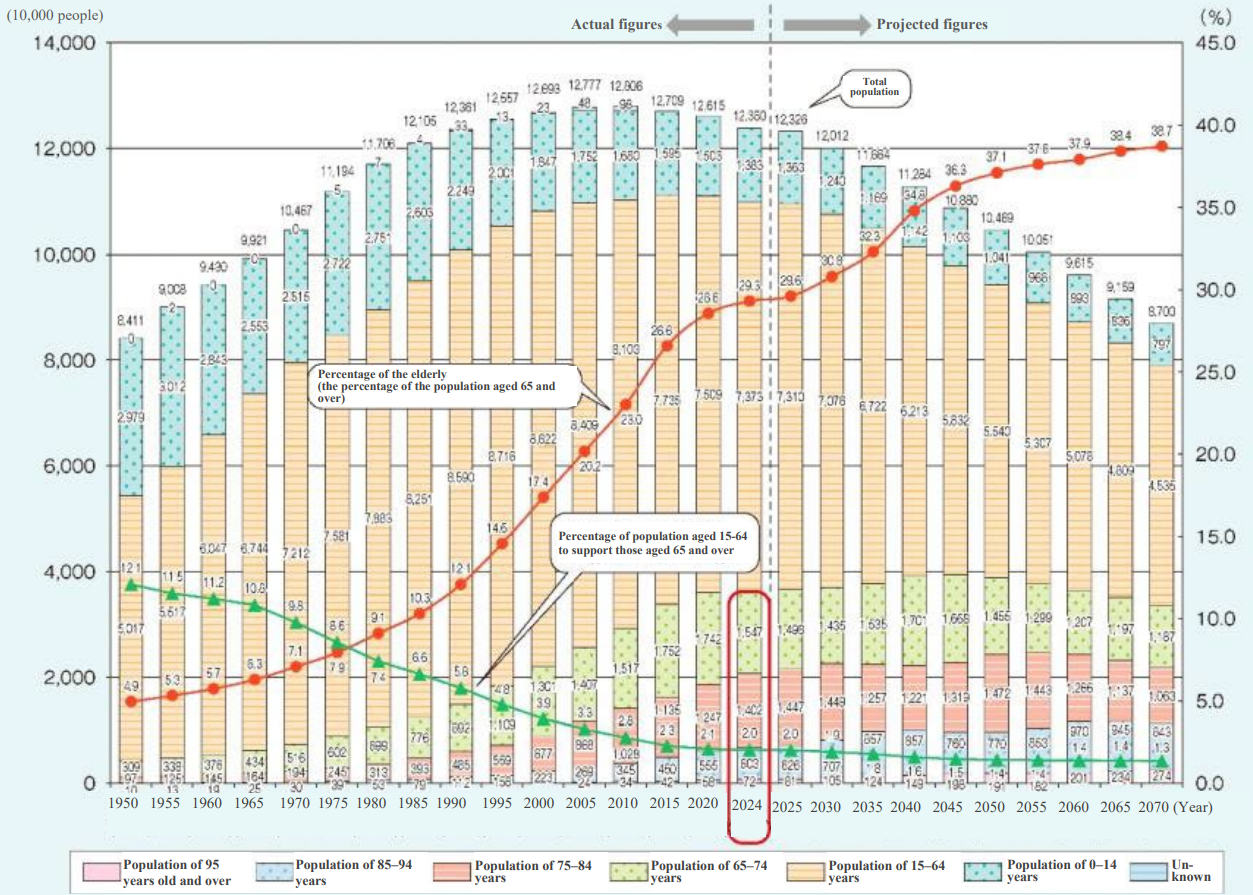
\includegraphics[width=0.75\linewidth]{fig/chp1/chp1_no_people.png}
    \caption{Trends in population ageing and future projections in japan\cite{cabinet_office_2025}}
    \label{fig:placeholder}
\end{figure}

この構造的な労働供給の縮小は，特に労働集約型産業である介護・家事支援サービス分野において顕著である．
厚生労働省の推計では，2040年度には約272万人の介護職員が必要となると予測されているが\cite{mhlw_caregiver_2024}，リクルートワークス研究所の報告によれば，現状のまま推移した場合，2040年には介護サービス職で約58万人の供給不足が生じると試算されている\cite{recruit_works_2024}．
このように増大し続ける支援需要と減少する労働供給の間の需給ギャップを埋めるため，ロボット技術による業務の代替・補完への期待はかつてないほど高まっており，サービスロボットの研究開発は喫緊の社会的要請となっている．

数ある家事支援の中でも，「料理（調理作業）」は特に重要性を持つ．
第一に，食事は生命維持と健康管理に直結する毎日数回の必須タスクであり，掃除や洗濯と比べて頻度が高い．
第二に，献立計画から食材の調達，下処理，加熱，配膳，後片付けに至るプロセスは，高度な身体的スキルと認知的負荷を同時に要求する．
特に高齢者にとって，刃物や火を扱う調理作業は身体機能の低下とともに危険を伴うようになり，自立生活を維持する上での最大の支障となりやすい．
したがって，単なる利便性向上を超え，介護と生活の質の維持の観点から，家庭内での調理を物理的に支援するロボットの実現が強く望まれている．

\subsection{産業用と家庭用ロボットの差異}

料理ロボットの研究開発は，その利用する場が「産業（工場）」か「家庭」かによって，求められる機能や設計思想が根本的に異なる．
食品工場などの産業現場では，調理プロセスの自動化が既に高度に進展しているが，これらは環境と対象物が厳密に管理された「構造化環境」を前提としている．

産業用ロボットのアプローチは「タスクの特化」にある．
例えば，ジュースの充填（液体），パン生地の混練（粘弾性体），魚の切り身の加工（柔軟物）など，ロボットにとって扱いが難しいとされる対象物であっても，工場ではそれぞれの作業に最適化された専用機械やライン（ベルトコンベアシステム等）を用いることで処理を実現している．
ここでは，単一の作業を大量に繰り返す「生産効率」が最優先され，そのために広いスペースや専用の大型設備を用いることが許容される．
つまり，産業用ロボットは，環境側をロボットに合わせて固定・管理することで，複雑な認識や適応的な制御を最小限に抑え，高効率な自動化を達成しているのである．

一方，一般家庭のキッチンで稼働するサービスロボットには，産業用とは対照的な「非構造化環境」への適応が求められる（表\ref{tab:robot_comparison}参照）．

% \begin{table}[ht]
%   \centering
%   \caption{産業用ロボットと家庭用ロボットの特徴と比較}
%   \label{tab:robot_comparison}
%   \begin{tabularx}{\textwidth}{@{}lXX@{}}
%     \toprule
%     比較項目 & 産業用ロボット（工場） & 家庭用ロボット（キッチン） \\
%     \midrule
%     \textbf{環境} & \textbf{構造化環境} \newline 照明・配置が厳密に管理・固定 & \textbf{非構造化環境} \newline 未知で動的に変化する実世界 \\
%     \midrule
%     \textbf{アプローチ} & \textbf{タスク特化} \newline 液体・粉末等は専用機械で処理 & \textbf{タスク汎用性} \newline 1台のロボットで全工程を処理 \\
%     \midrule
%     \textbf{対象物} & \textbf{性状を問わず，対象ごとに専用機構で取り扱う}  & \textbf{形状不定・柔軟物} \newline 個体差が大きく未知のものが多い \\
%     \midrule
%     \textbf{制約条件} & \textbf{大規模な専用スペース・設備が可能} & \textbf{人間と共存する限られた空間} \newline 省スペース性が必須 \\
%     \midrule
%     \textbf{優先指標} & \textbf{生産効率・速度} \newline 1秒間に何個処理できるか & \textbf{適応力・汎用性} \newline 未知の状況に対応できるか \\
%     \bottomrule
%   \end{tabularx}
% \end{table}
\begin{table}[ht]
  \centering
  \caption{Comparison between Industrial and Domestic Robots}
  \label{tab:robot_comparison}
  \begingroup
  \footnotesize
  \setlength{\tabcolsep}{4pt}
  \renewcommand{\arraystretch}{0.95}
  \begin{tabularx}{.95\textwidth}{@{}lXX@{}}
    \toprule
    Item & Industrial Robots & Domestic Robots \\
    \midrule
    \textbf{Environment}
    & \textbf{Structured} \newline Lighting and object placement are controlled
    & \textbf{Unstructured} \newline Conditions are unknown and dynamically changing \\
    \midrule
    \textbf{Approach}
    & \textbf{Task-specific} \newline Dedicated machines are used for each process
    & \textbf{Versatile} \newline A single robot handles multiple processes \\
    \midrule
    \textbf{Objects}
    & \textbf{Dedicated handling} \newline Objects are handled according to their properties
    & \textbf{Irregular and deformable} \newline Objects vary widely and are often unknown \\
    \midrule
    \textbf{Constraints}
    & \textbf{Dedicated space} \newline Large-scale equipment can be used
    & \textbf{Shared limited space} \newline Space-saving design is required \\
    \midrule
    \textbf{Priority}
    & \textbf{Efficiency and speed} \newline Processing quantity per unit time
    & \textbf{Adaptability} \newline Response to unknown situations \\
    \bottomrule
  \end{tabularx}
  \endgroup
\end{table}

\begin{enumerate}
    \item \textbf{スペースの制約：} 一般家庭には工場のような専用ラインや大型機械を設置する空間的余裕はないため，人間と共存できるサイズ（省スペース性）が必須となる．そのため，1台（あるいは双腕）のロボットアームとハンドを用いて，切るや炒める皮をむくといった，運動学的にも力学的にも性質の異なる多種多様な調理動作を，同一のハードウェアで遂行する能力が求められる．
    
    \item \textbf{対象物の不確実性と多様性：} 家庭内の食材は工業製品とは異なり，極めて高い「個体差」を持つ．同じ「ジャガイモ」であっても，その形状・大きさ・表面の凹凸・硬さは一つ一つ異なる個体差を持つ．また，調理器具や食器も規格化されておらず，未知の形状をした対象物を即座に認識し，適切に扱う能力が要求される．

    \item \textbf{道具・設備の非標準化（人間中心設計への適応）：} 工場ではロボット専用のハンドや治具が用いられるが，家庭では人間用に設計された既存の調理器具（包丁，ピーラー，鍋など）をそのまま利用しなければならない．ロボットは，自身の身体構造と関係なく作られた道具を把持し，その幾何学的・力学的機能を理解して操る能力が求められる．

    \item \textbf{センシング環境の悪条件：} 均一な照明が保証される工場とは異なり，家庭のキッチンでは，ステンレスの反射，水やガラスなどの透明物体，湯気による遮蔽など，視覚センサにとってのノイズ要因が極めて多い．不完全な点群データからでも，対象の物理モデルをロバストに再構成・推定する能力が必要となる．
\end{enumerate}


こうした困難な制約に対し，Miso RoboticsのFlippy\cite{miso2025flippy_nextgen}やMoley Roboticsのシステムなど，先駆的な取り組みが進められている．
しかし，これらの多くは依然として「専用設計された環境」や「規格化された手順」に依存している．
業務用のシステムは食材供給を固定化し，家庭用の既存システムも専用レシピや器具を前提とする場合が多い．
したがって，未知の食材や道具に対してその場で判断し適応する，真の意味での「非構造化環境への適応力」が，家庭用料理ロボット実現の鍵となる．

これらの家庭環境特有の課題は，ロボットによる物理的なマニピュレーションの観点から抽象化すると，本質的に（i）形状の多様性，（ii）力学的相互作用の複雑さ，（iii）環境・道具による拘束，という3つの「物理的制約」として整理できる．


\section{課題と提案手法}

\subsection{家庭環境での困難性}

前述の通り，家庭環境での適応性を実現するためには，調理作業に内在する以下の3つの物理的制約を克服する必要がある．

\begin{enumerate}
    \item \textbf{形状の多様性への適応（幾何学的不確実性）：} 食材の形状は不定形であり，事前に正確なモデルを用意することは不可能である．従来の剛体マニピュレーションで主流であった，既知のCADモデルとのマッチングに基づく姿勢推定や把持計画をそのまま適用することはできない．したがって，ロボットはセンサの点群情報から対象の局所的な表面曲率や法線ベクトルといった幾何特徴を即座に抽出し，個体差に合わせてオンラインで動作軌道を生成する能力が求められる．
    
    \item \textbf{複雑な力学的相互作用：} 調理は単なる物体の移動（ピックアンドプレース）ではなく，対象の物理的変形や状態変化を伴う．特に，包丁による「切断」やピーラーによる「皮むき」は，対象物の塑性変形や破壊を伴う不可逆なプロセスである．これらを成功させるためには，単なる位置制御ではなく，対象の硬さに応じた反力制御，皮むき時の接触圧維持など，実行時の接触状態に基づいた「力」の能動的な管理（インピーダンス制御等）が不可欠である．
    
    \item \textbf{環境・道具による拘束（ツール媒介操作の複雑性）：} ロボットは食材を直接操作するだけでなく，包丁，ピーラー，容器といった「道具（環境）」を介して間接的に作用させる．道具を使用する作業においては，ロボットのハンド，道具，対象物，そしてまな板の間に複雑な運動学的・力学的な拘束が生じる．道具が持つ幾何的な機能（例：容器の容積）や力学的な制約（例：刃が滑らない角度）を理解し，環境全体の物理モデルとして動作に反映させる必要がある．
\end{enumerate}

これらの困難性は，料理タスクが単なる視覚的なパターン認識や事前の軌道ティーチングだけでは解決できず，対象と環境に対する深い「物理的推論」を必要としていることを示している．
したがって，これらの物理的推論をロボットシステム上で実装可能な形で行うためには，実世界の対象と環境を，物理法則を適用できる「計算可能な内部表現」への落とし込むことが不可欠となる．

\subsection{提案手法：3Dモデルを基盤とした「分析主導型」アプローチ}

前節で述べた「形状・力・環境」という3つの物理的制約に対応するため，本研究ではRGB-Dセンサ等から得られる「3Dモデル」を物理世界の計算代理として構築し，それに対する多角的な「分析」を通じて適応的な「動作を生成する」統一的なアプローチ（図\ref{fig:topflow}）を提案する．

\begin{figure}[t]
    \centering
    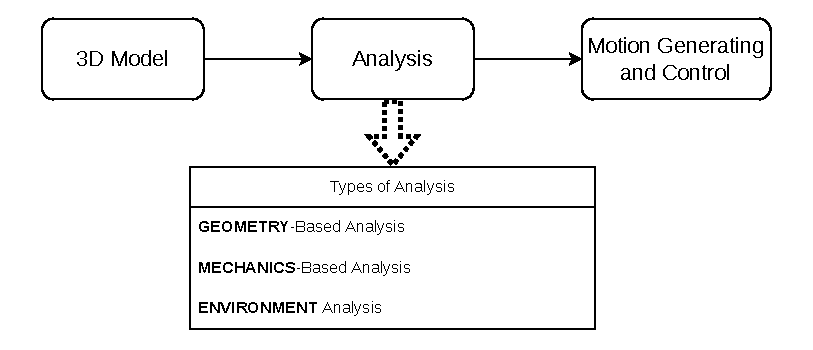
\includegraphics[width=.95\linewidth]{fig//chp1/DoctoralThesis_TopFlow.drawio.pdf}
    \caption{The flow of proposed approach}
    \label{fig:topflow}
\end{figure}

本研究において「3Dモデル」とは，主にRGB-Dセンサから取得された点群データを指し，必要に応じてメッシュ化や幾何プリミティブへのフィッティング処理が施されたものを意味する．
このモデルに対し，以下の3つの観点から分析を行うことで，前述の課題を解決する．

\begin{enumerate}
    \item \textbf{幾何学的な分析：} 対象物の3D形状（法線，体積など）を解析し，その形状的特徴に合わせてロボットの軌道を生成する．これは「形状の多様性」への直接的な解となる．
    
    \item \textbf{力学的な分析：} 3Dモデル上で，切断時の反力，摩擦，モーメントの釣り合いを解析・シミュレーションする．これにより「複雑な力学的相互作用」における動的な安定性を実現する．
    
    \item \textbf{環境的な分析：} 食材単体ではなく，容器や刃物といった「環境（道具）」との幾何的・力学的関係性を解析する．これにより「環境・道具による拘束」を考慮した間接的な操作が可能となる．
\end{enumerate}

また，本アプローチでは，分析によって導出された動作計画を基本とし，必要に応じて力覚センサ等を用いたフィードバック制御を併用する．
すなわち，3Dモデル上の分析が大まかな「解」を与え，実世界での接触情報が微細な誤差を吸収するという階層的な構造をとることで，ロバストなタスク遂行を保証する．

本論文が提案するのは，あくまで「3Dモデル上の分析から動作パラメータを導出する」という設計アプローチであり，あらゆる料理タスクを全自動化する単一のシステムではない．
しかし，このアプローチは多様な物理的制約を持つタスクに対して汎用的に適用可能である．

\section{目的と検証タスクの選定}

\subsection{本論文の目的}

% 本論文の目的は，RGB-D点群から構築した3Dモデルにより作業環境および対象物を表現し，その幾何・物理的特徴に基づく推論を通じて，動作と制御の設計を行う汎化可能な操作設計のアプローチを提示することにある．
% 具体的には，未知の食材や道具に対しても，その場で取得した3Dモデルに対する物理的な整合性の分析を行うことで，適応的な行動則を導出できることを示す．
本論文の目的は，RGB-D点群から構築した3Dモデルを計算基盤として，対象物および作業環境の幾何・物理的特徴を分析し，その結果をタスク固有の動作生成および制御設計へ接続する操作設計アプローチを提示することにある．
さらに，物理的相互作用の性質が異なる複数の料理操作に本アプローチを適用し，その有効性と適用可能性を検証する．
具体的には，形状が事前に与えられていない（以降は「未知」とよぶ）食材や道具に対しても，その場で取得した3Dモデルの幾何・物理的な特徴を分析することにより，対象に適応したロボットの動作生成および制御設計が可能であることを示す．

\subsection{検証タスクの選定}

提案する「分析主導型」アプローチの有効性を実証するため，本論文では物理的相互作用の特性が大きく異なる以下の3つのタスクを選定した．
これらは，料理作業における代表的な物理対象（流体・固形食材・道具）を含み，さらに状態変化（不可逆変形・破壊）と接触/環境制約を主要な観点としてカバーするように設計した．

% \begin{table}[htbp]
%   \centering
%   \caption{検証タスクと適用される分析手法の対応}
%   \label{tab:tasks}
%   \begin{tabular}{@{}cccc@{}}
%     \toprule
%     検証タスク & 1. 幾何学的な分析 & 2. 力学的な分析 & 3. 環境的な分析 \\
%     \midrule
%     \textbf{タスク1：皮むき} &  法線・軌道 & 実行中接触圧維持 & ------ \\
%     \addlinespace
%     \textbf{タスク2：注ぐ} &  容積・形状 & ------ &  容器間関係 \\
%     \addlinespace
%     \textbf{タスク3：安定把持} &  把持点探索 &  力学解析 &  道具拘束 \\
%     \bottomrule
%   \end{tabular}
% \end{table}
\begin{table}[htbp]
  \centering
  \caption{Correspondence between validation tasks and applied types of analysis}
  \label{tab:tasks}
  
  \scriptsize
  \setlength{\tabcolsep}{4pt}
  \renewcommand{\arraystretch}{0.95}
  \begin{tabularx}{.95\textwidth}{@{}cccc@{}}
    \toprule
    Validation Task & 1. Geometric Analysis & 2. Mechanics-Based Analysis & 3. Environmental Analysis \\
    \midrule
    \textbf{1st: Peeling} & Surface Normals and Trajectory & Contact Pressure Maintenance & ------ \\
    \addlinespace
    \textbf{2nd: Pouring} & Volume and Shape & ------ & Inter-Container Relationship \\
    \addlinespace
    \textbf{3rd: Holding} & Holding Point Search & Mechanics-Based Evaluation & Tool Constraints \\
    \bottomrule
  \end{tabularx}
\end{table}

\begin{enumerate}
    \item \textbf{タスク1：皮むき動作（不規則形状への幾何的適応と接触維持）} \\
    このタスクは，個体差の大きい「不規則な曲面形状」への適応能力を検証する．3Dモデルを用いた\textbf{「幾何学的な分析」}により最適な刃の軌道を生成し，実行時の力制御でモデル誤差を吸収することで，形状の不確実性に対応できることを示す．
    
    \item \textbf{タスク2：注ぎ動作（容器という「環境」を利用した流体操作）} \\
    このタスクは，直接把持できない「流体」の操作能力を検証する．対象物そのものではなく，容器の3Dモデルに対する\textbf{「環境的な分析」}（容積推定や流出特性の解析）と\textbf{「幾何学的な分析」}を行うことで，外部計量器具なしに定量的な操作が可能であることを示す．
    
    \item \textbf{タスク3：安定把持（外力に抗する力学的・環境的推論）} \\
    このタスクは，切断という「大きな外力」および包丁という「道具」が存在する状況下での高度な推論能力を検証する．3Dモデル上で想定される切断力や摩擦力をシミュレーションする\textbf{「力学的な分析」}と，包丁やまな板との関係を考慮する\textbf{「環境的な分析」}を統合し，最適な把持戦略を導出できることを示す．
\end{enumerate}

\subsection{本論文の寄与}

本論文の主な寄与は，アプローチの提案，タスク固有アルゴリズムの開発，および実ロボットシステムでの実証という観点から，以下の3点に要約される．

\begin{enumerate}

\item \textbf{アプローチの確立（3Dモデルベースの分析主導型設計）} \\
非構造化環境における料理タスク群に対し，RGB-D点群から構築した3Dモデルを物理世界の「計算代理」と位置づけ，そこでの幾何学的・力学的・環境的な分析を通じて適応的な動作と制御パラメータを導出する「分析主導型」の操作設計アプローチを提案した．これにより，従来多く用いられてきた発見的ルールや事前ティーチングに依存する方法に対し，物理法則に基づく動作設計のための体系的な設計指針を与える．

\item \textbf{具体的アルゴリズムの開発（料理操作における代表的物理相互作用への適用）} \\
提案する設計手法を，物理的特性が大きく異なる3つの料理タスク（皮むき，注ぐ，切断把持）に適用し，それぞれのタスクを解決するための具体的なアルゴリズムを開発した．具体的には，(a) 不規則形状の食材に対する幾何学的軌道生成と力覚制御を統合した皮むき手法，(b) 未知容器の3D幾何および環境推論に基づく定量注液手法，(c) 包丁からの外力と環境拘束を考慮した力学解析による安定把持点探索手法を提案した．

\item \textbf{実機実験による検証（実ロボットによる未知対象操作の検証）} \\
開発した手法を双腕ロボットシステムに実装し，事前の精密なCADモデルを与えられていない未知の食材や容器に対しても提案手法が適用可能であることを実験により確認した．

\end{enumerate}

\section{本論文の構成}


本論文は全7章で構成される．
第2章では，調理ロボットに関連する先行研究を概観する．
産業用ロボットのアプローチと，家庭用ロボットに求められる非構造化環境への適応に関する研究動向を整理し，本研究の立ち位置を明確にする．
第3章では，本研究の基礎となる3Dモデルの取得手法，および実験プラットフォームの構築について述べる．
RGB-Dセンサを用いた点群取得，前処理，モデル化のプロセスと，その精度検証について詳述する．
第4章では，「皮むく」タスクを通じ，3Dモデルの表面幾何解析による軌道生成と力覚フィードバックの統合手法について論じ，その有効性を検証する．
第5章では，「注ぐ」タスクを通じ，容器の3Dモデルを用いた幾何学的推論（容積計算）に基づく流体操作手法について論じ，その有効性を検証する．
第6章では，「安定把持」タスクを通じ，包丁からの外力に対する力学解析と環境解析を統合した把持計画手法について論じ，その有効性を検証する．
最後に第7章において，本論文を総括し，今後の展望を述べる．
以上の構成により，第3章で三つのタスクに共通する計測・モデリング基盤を示し，第4章から第6章で，皮むき，定量注ぎ，および切断中の安定把持という三つの研究課題を順に検証する．
各検証章では，第1章で示した「3Dモデル，分析，動作計画・制御」の関係を同一の観点から整理し，最終章で得られた知見と適用範囲を総括する．




